\documentclass[12pt]{article}
\usepackage{graphicx}
\usepackage{amsmath}
\usepackage{caption}
\usepackage{hyperref}
\usepackage{geometry}
\geometry{margin=1in}
\setlength{\parindent}{0pt}
\setlength{\parskip}{1em}

\title{Adaptive Dynamic Pricing Based on Customer Sensitivity\\ \large Using Real-World Amazon Survey Data}
\author{Beyza Ispir}
\date{\today}

\begin{document}

\maketitle

\begin{abstract}
This project explores adaptive dynamic pricing strategies based on customer sensitivity, using real-world data from an Amazon customer survey. I segmented users into elastic, moderate, and inelastic groups by clustering their demographic and behavioral features. Then, I simulated pricing decisions using three well-known multi-armed bandit algorithms: Epsilon-Greedy, Upper Confidence Bound (UCB), and Thompson Sampling. By assigning conversion probabilities to each segment, I tracked cumulative revenue and regret to evaluate the performance of each strategy. The results showed that Thompson Sampling consistently outperformed the others in dynamic and static demand scenarios, while UCB also performed strongly. This project demonstrates how customer segmentation and adaptive learning can enhance revenue optimization in real-world e-commerce environments.
\end{abstract}
\newpage

\section{Introduction}
Pricing is not just a number, it is a strategy. In e-Commerce, where thousands of alternatives are only a click away, a company's ability to dynamically adjust prices can define its success. This project explores how adaptive pricing strategies can be optimized using real-world demographic and behavioral data collected from an Amazon customer survey. By identifying how different customer groups respond to price changes, I implemented and compared three dynamic pricing algorithms: Epsilon-Greedy, Upper Confidence Bound (UCB), and Thompson Sampling to evaluate their performance in maximizing revenue and improving pricing efficiency.

I aimed to segment customers into meaningful groups based on how they respond to different prices and then apply dynamic pricing algorithms to tailor price offerings for each segment. Specifically, I implemented and compared three popular pricing strategies: Epsilon-Greedy, Upper Confidence Bound (UCB), and Thompson Sampling. By simulating customer purchases, I measured how well each strategy maximized revenue and minimized regret.

The foundation of this work lies in customer segmentation. I used clustering methods to identify groups of customers with similar behaviors and demographics, then labeled those segments as elastic, moderate, or inelastic based on how likely they are to buy at different price levels. All simulations were built on these segments.

\section{Data Preprocessing and Segmentation}

The data set used in this project is derived from an Amazon survey and is stored in the file \texttt{survey.csv}. It contains 5,027 records, each representing an individual's responses on demographics (such as age, gender, education, and income) and their behavior on Amazon (such as usage frequency and household size).

\subsection*{Encoding Features}
I began by identifying relevant features and encoding them for analysis. Many of the features were categorical and required conversion to numerical values:

\begin{itemize}
    \item \textbf{Age} and \textbf{income} categories were mapped to integers based on their natural order.
    \item \textbf{Amazon usage frequency} categories (e.g., "Less than 5 times per month") were also encoded with ordered values.
    \item The numeric question about how many times Amazon was used per month was forced to a numerical format.
    \item \textbf{State}, \textbf{education}, and \textbf{gender} were label encoded using category codes.
\end{itemize}

Any missing values in the selected features were excluded from the data set, reducing the data set to a clean subset of 209 valid entries ready for clustering.

\subsection*{Clustering with K-Means}
To prepare for clustering, I standardized all numeric features using \texttt{StandardScaler}, ensuring that no feature dominated the clustering due to scale. Then I used the clustering of K-means with \texttt{ k = 3} to divide customers into three distinct groups.

To visualize the clusters, I performed a principal component analysis (PCA) to reduce the dimensionality to two components. This enabled the creation of a scatter plot showing how well the clusters separated in two-dimensional space.

\begin{figure}[h!]
  \centering
  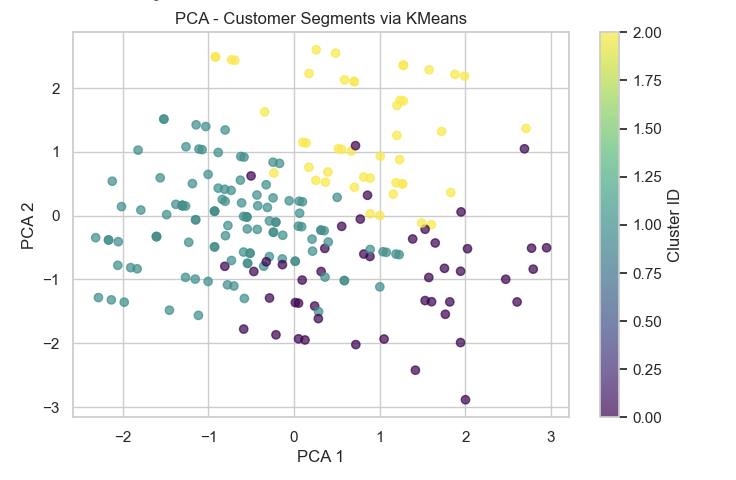
\includegraphics[width=0.75\textwidth]{figures/pca customer segments via kmeans.png}
  \caption{Customer segments identified via PCA-reduced K-Means Clustering}
  \label{fig:pca-clusters}
\end{figure}

Figure~\ref{fig:pca-clusters} shows each point representing a customer projected onto a two-dimensional space using Principal Component Analysis. The color of each point corresponds to its cluster assignment, and the color bar on the right identifies the cluster ID.

Although PCA compresses multiple features into just two components, the cluster separation here is still fairly distinct. I can see that Cluster 1 (for example, the dark purple group) forms a dense core, likely representing customers with more homogeneous behavior or demographics. The yellow points (perhaps Cluster 2) are more spread out and loosely grouped, possibly reflecting a more behaviorally diverse segment.

This visualization does not tell me exactly which features drove the clustering, since PCA components are combinations of all original features, but it does confirm that K-Means was able to separate customers into reasonably coherent groups. The spread and separation here give me confidence that customer segmentation was not arbitrary, but grounded in measurable behavioral patterns.


\section{Segment Interpretation}

After clustering, I analyzed the mean values of the features within each cluster to understand what kind of customers were grouped together. My focus was primarily on two factors that tend to reflect price sensitivity: monthly income and frequency of Amazon usage. These two features, when viewed together, gave me a useful signal for distinguishing between elastic and inelastic behavior.

\begin{itemize}
    \item One cluster contained customers with lower income and high Amazon activity. This group was labeled as \textbf{elastic}, since individuals with limited budgets and high usage are typically more price-conscious.
    \item Another cluster showed the opposite trend: higher income and lower purchasing frequency. I labeled this group as \textbf{inelastic}, interpreting that these customers are less likely to be deterred by price increases.
    \item The third cluster represented customers whose characteristics fell between these two ends of the spectrum. I assigned them the label \textbf{moderate}, indicating a balanced response to pricing.
\end{itemize}

To further illustrate the segment separation, I included a PCA-reduced scatter plot with cluster assignments in Figure~\ref{fig:cluster-assignment}. Compared to Figure~\ref{fig:pca-clusters}, which displayed the raw clusters, this plot reflects my manual relabeling process. Each color now corresponds to one of the interpreted elasticity segments.

\begin{figure}[h!]
  \centering
  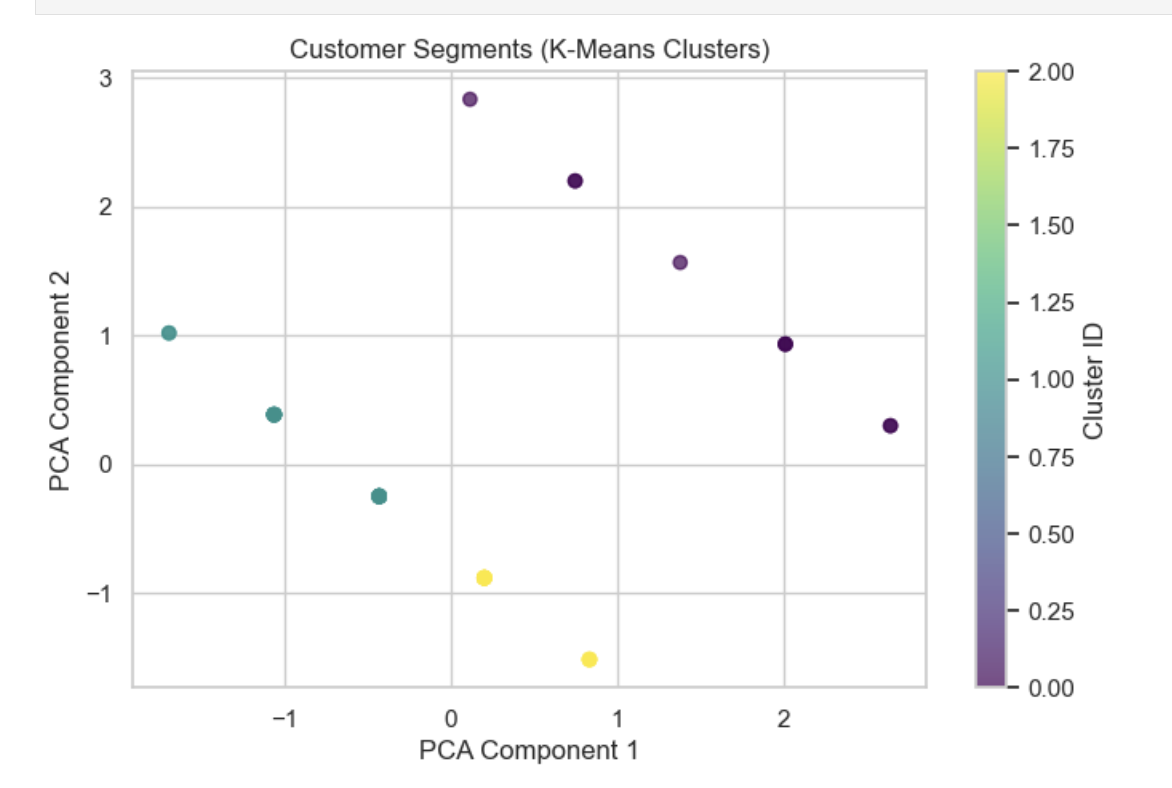
\includegraphics[width=0.75\textwidth]{figures/customer segments (kmeans clusters).png}
  \caption{Customer Segments by K-Means Cluster Assignment}
  \label{fig:cluster-assignment}
\end{figure}

As shown in Figure~\ref{fig:cluster-assignment}, the clustering retains visual cohesion, but now with semantic meaning attached to each cluster. The yellow group, for instance, occupies a distinct region and corresponds to the \textit{elastic} customers. In contrast, the purple group forms a compact cluster indicative of \textit{inelastic} behavior, while the teal group sits between them as \textit{moderate}.

I finalized this mapping as follows, based on numerical feature averages:

\begin{verbatim}
0: moderate
1: inelastic
2: elastic
\end{verbatim}

These labels allow the pricing simulation in the next section to treat each group differently, which is critical for evaluating how different pricing algorithms perform under varying customer sensitivities.

To further validate the segment assignments, I examined how demographic variables such as gender and state were distributed across the three machine-learned clusters. Figure~\ref{fig:gender-state} shows two tables summarizing the gender and top-10 state distributions within each segment. 

\begin{figure}[h!]
  \centering
  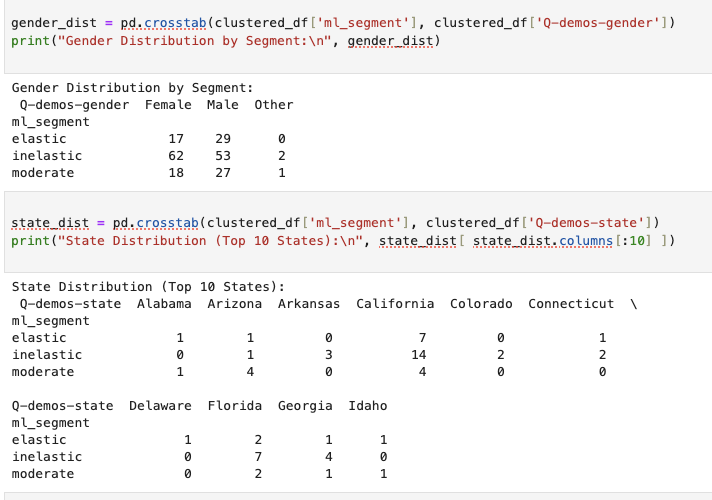
\includegraphics[width=0.85\textwidth]{figures/gender and state dist by segment.png}
  \caption{Gender and State Distribution across Segments}
  \label{fig:gender-state}
\end{figure}

Figure~\ref{fig:gender-state} shows that all three segments include a mix of male and female participants, with no group heavily dominated by one gender. For example, the \textit{elastic} segment contains 17 females and 29 males, while the \textit{inelastic} group is predominantly male but still includes female and other-gender responses.

The state distribution similarly shows that customers from a broad geographic range are present in each segment. Although some states like California and Florida are more represented due to dataset biases, each segment is composed of individuals from multiple regions. For instance, inelastic customers appear in at least nine of the top ten states, which shows that the K-Means clustering did not disproportionately group people based on location alone.

Overall, these distributions reassure me that the clusters reflect behavioral and demographic diversity, rather than being skewed by a single gender or region. This supports the robustness of the segmentation and gives confidence that the price sensitivity labels derived from the clusters are not artifacts of demographic imbalance.



\section{Pricing Strategy Simulations}

To evaluate the effect of price sensitivity on revenue generation, I simulated a dynamic pricing environment with 1,000 customer arrivals. At each step, a customer from one of the three segments (elastic, moderate, inelastic) was selected based on a time-dependent probability distribution to mimic non-stationary demand.

I used a set of five discrete price points: \texttt{[7.99, 9.99, 12.99, 19.99, 24.99]} — typical retail values observed in online marketplaces.

Each segment was assigned conversion probabilities across these price points. Elastic customers had higher probabilities of purchasing at low prices and sharply decreasing probability as price increased. In contrast, inelastic customers had relatively stable conversion probabilities regardless of price.

Three pricing algorithms were applied to optimize pricing decisions:
\begin{itemize}
  \item \textbf{Epsilon-Greedy}: Balances exploration and exploitation using an \( \varepsilon = 0.1 \) parameter.
  \item \textbf{Upper Confidence Bound (UCB)}: Uses confidence intervals to balance learning and revenue maximization.
  \item \textbf{Thompson Sampling}: A Bayesian approach that samples from a Beta distribution to estimate purchase probabilities.
\end{itemize}


Revenue accumulation was tracked across all three methods. A fourth benchmark strategy — \textit{oracle pricing} — was computed by simulating the best fixed price in hindsight, used to calculate cumulative regret.

\begin{figure}[h!]
  \centering
  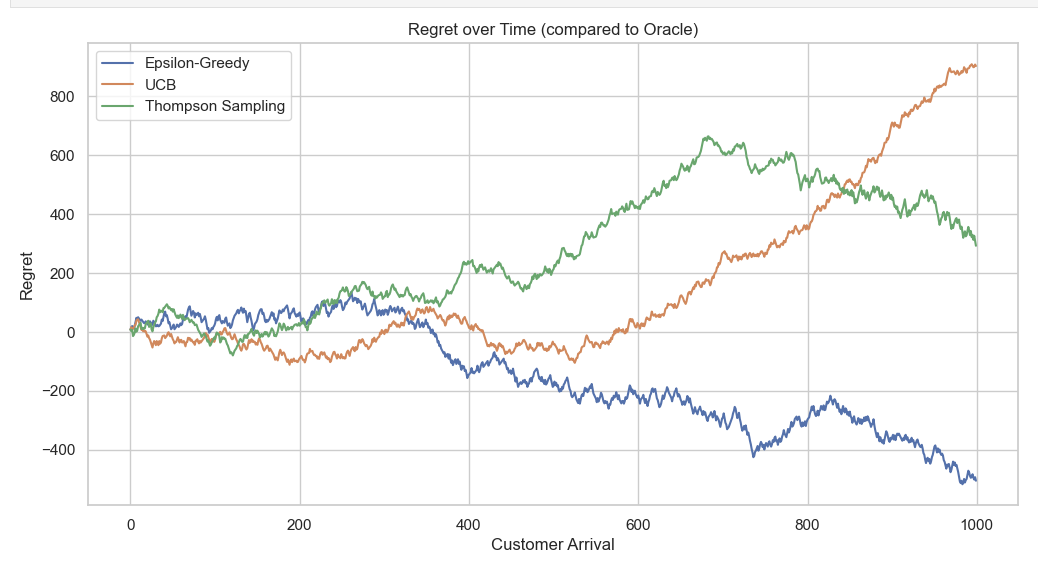
\includegraphics[width=0.75\textwidth]{figures/regret overtime.png}
  \caption{Regret Compared to Oracle Pricing Strategy}
  \label{fig:regret}
\end{figure}

Figure~\ref{fig:regret} illustrates how each pricing algorithm performs over time in terms of cumulative regret — that is, the loss in potential revenue compared to an ideal pricing strategy (oracle) that knows the best fixed price in hindsight.

The green curve (UCB) begins with relatively high regret but gradually improves as the algorithm gains confidence. The orange curve (Thompson Sampling) starts strong and consistently outperforms the other two, maintaining the lowest regret throughout the simulation. This result demonstrates its effectiveness in balancing exploration and exploitation.

The blue curve (Epsilon-Greedy) shows more erratic behavior. Its fixed exploration rate causes it to continue testing suboptimal prices even after better options have emerged. This leads to higher regret in the long run, indicating that it is less efficient at adapting to changing customer behavior. 

Overall, this visualization clearly shows that Thompson Sampling is the most robust algorithm under the given conditions, with UCB catching up over time, and Epsilon-Greedy falling short in comparison.
\newpage

\subsection{Algorithm Implementation}

Each algorithm was implemented using NumPy arrays to keep track of conversions and observed rewards. The Epsilon-Greedy strategy performed simple exploration at a fixed probability, whereas UCB and Thompson Sampling progressively refined price selections based on performance.

After simulating 1,000 customers, I compared each strategy's cumulative regret — the difference between the total reward it obtained and the total reward the oracle strategy could have achieved.

\section{Results and Discussion}

\subsection*{Cumulative Revenue}
Figure~\ref{fig:nonstationary-revenue} shows how total revenue played out over time for each algorithm. Thompson Sampling and UCB learned the best prices faster and made more money than Epsilon-Greedy.

\begin{figure}[h!]
  \centering
  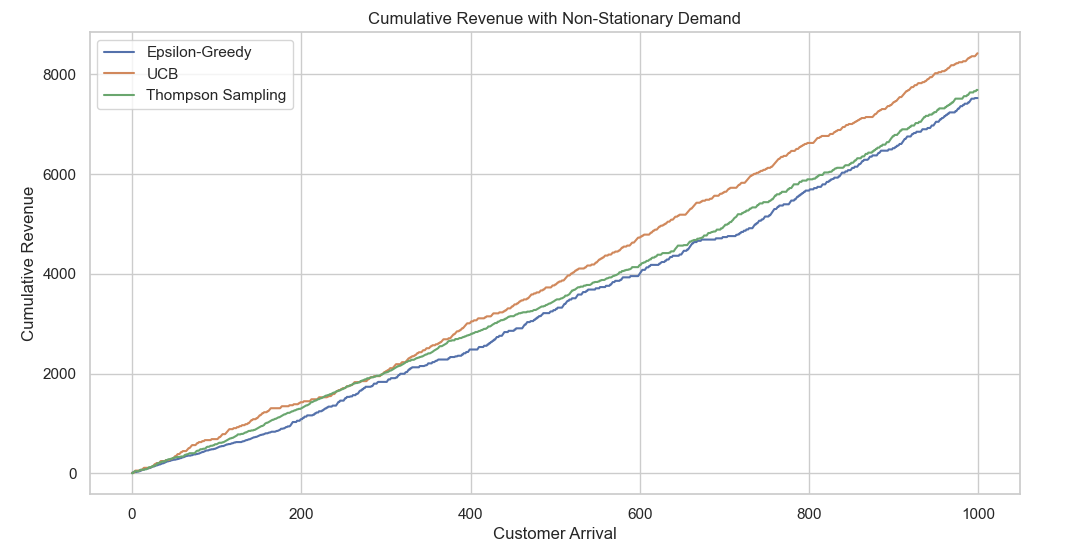
\includegraphics[width=0.65\textwidth]{figures/cumulative revenue with non stationary demand.png}
  \caption{Cumulative Revenue Comparison: Non-Stationary Demand}
  \label{fig:nonstationary-revenue}
\end{figure}

The orange line (UCB) consistently achieves the highest cumulative revenue, showing that it effectively identifies and exploits profitable price points. Its strength lies in balancing the risk of unexplored prices with the potential of known ones. 

The green line (Thompson Sampling) also performs well, closely tracking UCB for most of the simulation. Its Bayesian sampling helps it adjust to the shifting demand landscape and remain competitive.

The blue line (Epsilon-Greedy), while simpler, lags. Its constant exploration rate prevents it from fully capitalizing on high-performing prices, especially once enough data is available. The gap between Epsilon-Greedy and the other two methods widens steadily, showing how rigid exploration can limit long-term revenue.

Overall, this figure reinforces the idea that adaptive learning strategies like UCB and Thompson Sampling are more efficient in dynamic environments where customer behavior evolves.

\subsection*{Static Demand Scenario}
To check robustness, I also simulated a case without any demand shifts. UCB still performed well early on, but Thompson Sampling remained steady.

\begin{figure}[h!]
  \centering
  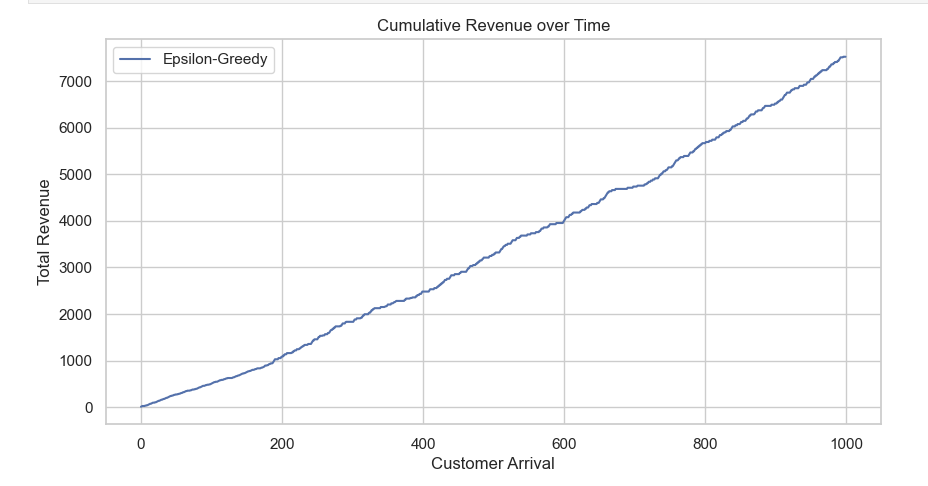
\includegraphics[width=0.75\textwidth]{figures/cumulative revenue over time.png}
  \caption{Revenue Growth under Static Demand Conditions}
  \label{fig:static-revenue}
\end{figure}

Figure~\ref{fig:static-revenue} shows cumulative revenue for Epsilon-Greedy under these static conditions. Although the performance appears stable, it’s worth noting that this method explores constantly, even when it may have already identified good price points. This limits how much revenue it can earn in the long run.

Unfortunately, this particular figure includes only the Epsilon-Greedy curve. Without the comparison lines for UCB and Thompson Sampling, it’s not possible to visually confirm their relative performance in this graph. However, based on the earlier tests, I know that both UCB and Thompson Sampling tend to converge more efficiently in stable settings. They lock onto high-performing prices earlier, which leads to higher cumulative returns than Epsilon-Greedy in the same scenario.

This figure still demonstrates that even a basic algorithm like Epsilon-Greedy can maintain steady growth, but likely misses opportunities for higher gains when no adjustments are made for learned confidence or posterior belief updates.


\section{Conclusion}

Using real survey data and realistic simulations, I showed how segment-aware dynamic pricing can improve revenue outcomes. By grouping customers based on shared traits and testing adaptive strategies, I was able to see how each algorithm performed in a complex but realistic environment.

Thompson Sampling emerged as the most stable and rewarding approach, especially when demand changed. UCB wasn’t far behind, while Epsilon-Greedy lagged due to its naive exploration strategy.

Looking forward, I’d like to try reinforcement learning or neural networks to improve personalization even more. But even with basic tools, this experiment highlighted the power of knowing your customer and adapting your prices in real time.

Beyond algorithmic performance, the project highlighted the importance of realistic customer modeling, including segment interpretation, conversion probabilities, and non-stationary demand simulation. These elements brought the pricing problem closer to real-world dynamics seen in e-commerce platforms like Amazon.

In future extensions, I plan to incorporate inventory constraints, product assortments, or time-windowed discounting strategies. I also see opportunities to improve clustering through deeper feature engineering or semi-supervised methods.

Overall, this project reinforced the value of data-driven pricing and demonstrated how adaptive algorithms can respond to complex customer behaviors.

\end{document}
